\section{Strålning genom glas}\label{sec:sunthroughwindowsmethod}

Flera olika metoder har använts vid beräkning av energiflöde genom fönster i byggnaden. Först beskrivs hur direkt solinstrålning genom fönster kan beräknas. Därefter följer ett kort stycke med redogörelser över hur man kan går tillväga för att beräkna energiflödet via svartkroppsstrålning mellan rummet och omgivningen. I avsnitt~\ref{subsec:otherradiation} beskrivs kortfattat ett par strålningssituationer som har försummats. Avslutningsvis presenteras en metod som används för att uppskatta hur mycket energi man kan spara genom att ta hänsyn till den direkta solinstrålningen.

\subsection{Solinstrålning}
För att beräkna den totala effekt som solstrålning tillför byggnaden via fönster behövs fönstrenas vinkelberoende g-värden, som presenteras i avsnitt~\ref{gvalue}. För att bestämma detta värde ur ekvation~\eqref{eq:radiationwindowstheory:gvalue} behöver parametern $z = \theta/90^\circ$ beräknas, där $\theta$ är vinkeln mellan solstrålingens riktning och fönstrets normal i grader. Detta görs genom att utgå från aktuellt datum och tid på dygnet.

En metod för att räkna ut solens position presenteras i \cite{walraven78} och en Matlabfunktion baserad på samma artikel kan ses i appendix \ref{app:sunposition}. Argumenten i denna funktion består av longitudinella och latitudinella koordinater för den aktuella platsen samt datum och tidpunkt. För Walleriusgatan är koordinaterna ungefär $12^\circ$ E respektive $58^\circ$ N.

När de azimuthala och altitudinella vinklarna, som här kallas $\beta$ och $\alpha$, relativt ett väderstreck respektive horisonten har beräknats, relateras infallsvinkeln mot glaset $\theta$ som

\begin{equation} 
\theta = \arccos{\left( \cos{\left(\beta - \gamma\right)}\cos{\left(\alpha\right)}\right)}
\end{equation}

där $\gamma$ är vinkeln mellan fönstrets normal och väderstrecket mot vilken den azimuthala vinkeln anges. Detta görs med funktionen angletheta i appendix \ref{app:sunwindows}.

Med dessa samband tillgängliga kan effektflödet på grund av solstrålning genom fönster beräknas, vilket kan göras med funktionerna \textit{gvalue} samt \textit{effekt} från appendix \ref{app:sunwindows}. Nödvändiga argument för dessa funktioner är g-värdet vid vinkelrätt infallande strålning samt konstanterna $p$ och $q$ från ekvation~\eqref{eq:gconstants}. % Repetera ekvationen?

För att ge ett exempel på hur effekten varierar med solintensiteten måste det byggas upp en approximativ funktion som beskriver solens intensitet vid marknivå som funktion av vinkeln över horisonten. Om vi antar att intensiteten är $I_o = \unit[1370]{Wm^{-2}}$\cite{physicshandbook} utanför atmosfären kan detta beskrivas med ett exponentiellt samband, $I = I_oe^{-\mu x}$ där $\mu$ kallas för atmosfärens absorbtionskoefficient som sätts till $\mu\approx \unit[4.6\cdot 10^{-5}]{m^{-1}}$ och $x$ är atmosfärens tjocklek mellan betraktaren och solen, i meter. Atmosfären antas dessutom vara som en homogen heltäckande sfär runt jorden och ungefär $\unit[15]{km}$ tjock, i positiv radiell riktning, överallt på jordens yta. $x$ kan nu beskrivas med solens höjd över horisonten, och ges av

\begin{equation}
x = R\cos{(90^\circ+\alpha)} + \sqrt{\left(R\cos{(90^\circ+\alpha)}\right)^2 + \left( R+\unit[15]{km}\right)^2 - R^2}
\end{equation}

där $\alpha$ är vinkeln mellan horisonten och solen och $R\approx\unit[6,731\cdot 10^6]{m}$ betecknar jordens radie \cite{physicshandbook}. Detta följer ur cosinussatsen. % Källa på siffran mu?

\paragraph{Inverkan av skuggor, rummets interiör och dylikt}

Sambanden ovan gäller då all strålning som passerar rutan stannar i rummet. Svårigheter uppstår när exempelvis persienner används. Dessutom har ingen hänsyn tagits till det faktum att omkringliggande byggnader kommer att blockera den direkta solstrålningen vid vissa tidpunkter.

Hur mycket av solinstrålningen som blockeras av persienner och gardiner är oerhört svårt att räkna ut. För det första är den parametern vinkelberoende, det vill säga beroende på persiennens konfiguration, färg och vinkel kommer olika mycket solstrålning att reflekteras tillbaka ut ur fönstret. För det andra måste hänsyn tas till mänskliga faktorer. Naturligtvis kommer vinkeln på persiennen att förändras vid godtyckliga tidpunkter. För att modellera sådana anordningar kan man enligt \cite{ASHRAE09} lägga till en vinkelberoende faktor, $0 \le R_\text{ref}\left( \theta \right) \le 1$, i \eqref{eq:totalsun} så att den slutliga formeln för solinstrålning genom fönster blir


\begin{equation}\label{eq:totalsunblinds}
Q = R_\text{ref}\left( \theta \right) \cdot g\left( \theta \right) \cdot A \cdot I_0 \cos{\theta} \unit[]{W}.
\end{equation}

Vid exempelberäkningarna i nästa avsnitt har dock ingen hänsyn tagits till denna koefficient  $R_\text{ref}$.

Effekten av skuggorna som orsakas av grannbyggnader i området kan också tas med i beräkningarna genom att mäta geometrin på omgivande byggnader. Detta behandlas dock inte inom det här projektet.

\subsection{Långvågsstrålning}\label{subsec:IRmethod}

Vid beräkning av energiflödet på grund av långvågig strålning antas att luften precis innanför fönstret håller konstant temperatur, $\unit[20]{^{\circ}C}$ och att de ''synliga'' ytorna utanför fönstret håller en temperatur motsvarande utomhustemperaturen, $T_\text{ute}$. Enligt beräkningen i avsnitt~\ref{IR} kommer 75\% av den infallande strålningen passera ett treglasfönster. Med detta i åtanke leder Stefan-Boltzmanns lag, \eqref{eq:boltzmanslag}, till, om interiören antas stråla som en svartkropp, att $q_\text{IR} = 0,75 \cdot \sigma [\left( (\unit[293]{K})^4 - T_\text{ute}^4\right)]\unit{W~m^{-2}}$. Den totala effekt som flödar ut på grund av svartkroppsstrålning blir då $q_\text{IR}\cdot A,~[W]$, där $A$ är den totala arean av fönsterglas på byggnaden.

\subsection{Övriga strålningseffekter}\label{subsec:otherradiation}

Då solen skiner kommer en viss andel direkt solstrålning att reflekteras från omgivande byggnader, växtlighet och dylikt för att sedan öka på intensiteten mot fönsterrutorna. Eftersom en andel av den direkt infallande solstrålningen genom fönsterrutorna även kommer att reflekteras mot rummens interiör och stråla ut igen har vi valt att inte ta hänsyn till dessa flöden, som beror starkt på omgivningens och interiörens utformning.

\subsection{Soltimmar under dygnet}
\label{subsec:sunhours}
Under året varierar antalet soltimmar. Detta kommer av att jordens rotationsaxel är vinkelrät 
mot jordens omloppsbana runt solen. I praktiken innebär detta att det är färre soltimmar
under vinterhalvåret och fler under sommarhalvåret. Då jordens bana kring solen är nästan
cirkulär kan vi approximera antalet soltimmar per dygn som en trigonometrisk funktion.
För Göteborg approximerar vi att årets kortaste dag är $\unit[6]{ timmar}$ och $\unit[32]{minuter}$ och årets längsta
dag är $\unit[17]{ timmar}$ och $\unit[28]{ minuter}$\cite{sunup}. Sedan noteras att dagen är som kortast vid vintersolståndet, runt den $20$
december.
Detta tillåter oss då att teckna dygnets soltimmar $\tau$ som ekvation~\eqref{eq:sunhours}. Här
är $t$ tiden i månader där $t=0$ motsvarar första januari och $t$ är periodiskt med perioden $12$ månader.

\begin{equation}
\label{eq:sunhours}
\tau = 12 - \left(6-\frac{32}{60}\right)\cos\left[\frac{\pi}{6}\left(t+\frac{1}{3}\right)\right]
\end{equation}

Fastigheten som detta arbete undersöker har en eldningsperiod från början av oktober till slutet av april. Därför önskas det att beräkna hur många soltimmar det i snitt är per dag under denna period. För detta syfte tecknas medelvärdet för antalet ljusa timmar per dag under eldningssäsongen $\bar{\tau}$ enligt

\begin{equation}
\label{eq:taubar}
\bar{\tau}= \frac{ \int^{16}_9 \left(12 - \left[6-\frac{32}{60}\right]\cos\left[\frac{\pi}{6}\left(t+
\frac{1}{3}\right)\right]\right)\mathrm{d}t}{\int^{16}_9 \mathrm{dt}}
\end{equation}

När ekvation~\eqref{eq:sunhours} och \eqref{eq:taubar} evaluerades gavs 
resultatet som kan ses i figur~\ref{fig:sunhours}.
Medelvärdet har här beräknats till $\bar{\tau}=\unit[9,39]{~timmar~per~dygn}$.
\begin{figure}
\centering
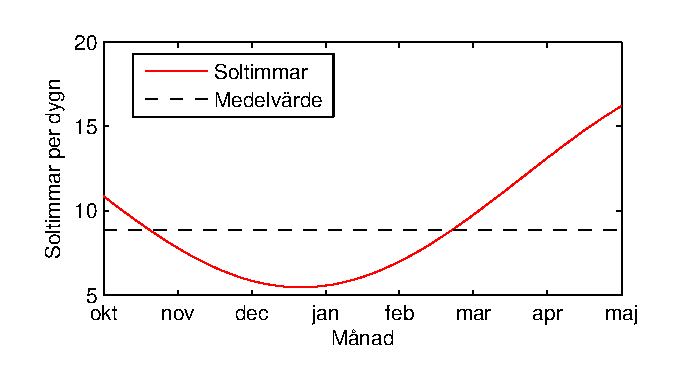
\includegraphics{images/sunhours.eps}
\caption{Antal timmar på ett dygn då solen är ovanför horisonten beräknat för månaderna under eldningsperioden.
Här är medelvärdet markerat med en streckad linje. Medelvärdet har beräknats vara
$\bar{\tau}=\unit[9,39]{~timmar~per~dygn}$.}
\label{fig:sunhours}
\end{figure}

\noindent
För att uppskatta hur mycket energi som går att spara genom att ta hänsyn till solen kommer arbetet
senare att behandla en decemberdag. Denna dag har behandlats under de två antagandena att den är solig respektive att den är molnig. Vi benämner energiåtgången för att värma fastigheten för den molniga dagen som $Q_\text{H}$ och energiåtgången för uppvärmning den soliga dagen som 
$Q_\text{L}$. Värden på dessa kommer sedan att användas tillsammans med
ovanstående beräkningar för att uppskatta den totala mängden energi som kan sparas. 

Från SMHI:s väderstatistik går det att utläsa att $\unit[8]{\%}$ av eldningsperiodens timmar är soliga\cite{SMHIdata}.
Detta motsvarar då $\unit[1,92]{~soliga~timmar}$ i snitt per dygn. Härnäst betecknas andelen timmar som är soliga som
$p = 1,92/\bar{\tau} = 1,92/9,39 = \unit[20,45]{\%}$. Nu beräknas medelenergiåtgången per dygn $Q$ enligt

\begin{equation}
Q = (1-p)\cdot Q_\text{H} + p\cdot Q_\text{L}.
\end{equation}

Slutligen kan kvoten $Q/Q_\text{H}$ beräknas vilket ger ett uttryck för hur stor andel av energin det går att spara

\begin{equation}
\frac{Q}{Q_\text{H}} = \frac{(1-p)\cdot Q_\text{H} + p\cdot Q_\text{L}}{Q_\text{H}} = 1-p+p\frac{Q_\text{L}}{Q_\text{H}}.
\end{equation}
